%%%%%%%%%%%%%%%%%%%%%%%%%%%%%%%%%%%%%%%%%
% American Geophysical Union (AGU)
% LaTeX Template
% Version 1.0 (3/6/13)
%
% This template has been downloaded from:
% http://www.LaTeXTemplates.com
%
% Original author:
% The AGUTeX class and agu-ps referencing style were created and are owned 
% by AGU: http://publications.agu.org/author-resource-center/author-guide/latex-formatting-toolkit/
%
% This template has been modified from the blank AGU template to include
% examples of how to insert content and drastically change commenting. The
% structural integrity is maintained as in the original blank template.
%
% Important notes: 
% This template retains extensive commenting from the AGU template. It is heavily 
% advised you read these comments and follow them in order to insure a speedy 
% submission process.
%
%%%%%%%%%%%%%%%%%%%%%%%%%%%%%%%%%%%%%%%%%

%%%%%%%%%%%%%%%%%%%%%%%%%%%%%%%%%%%%%%%%%%%%%%%%%%%%%%%%%%%%%%%%%%%%%%%%%%%%
% AGUtmpl.tex: this template file is for articles formatted with LaTeX2e,
% Modified March 2013
%
% This template includes commands and instructions
% given in the order necessary to produce a final output that will
% satisfy AGU requirements.
%
% PLEASE DO NOT USE YOUR OWN MACROS
% DO NOT USE \newcommand, \renewcommand, or \def.
%
% FOR FIGURES, DO NOT USE \psfrag or \subfigure.
%
%%%%%%%%%%%%%%%%%%%%%%%%%%%%%%%%%%%%%%%%%%%%%%%%%%%%%%%%%%%%%%%%%%%%%%%%%%%%
%
% All questions should be e-mailed to latex@agu.org.
%
%%%%%%%%%%%%%%%%%%%%%%%%%%%%%%%%%%%%%%%%%%%%%%%%%%%%%%%%%%%%%%%%%%%%%%%%%%%%

% Step 1: Set the \documentclass

% There are two options for article format: two column (default) and draft.

% PLEASE USE THE DRAFT OPTION TO SUBMIT YOUR PAPERS.
% The draft option produces double spaced output.

% Choose the journal abbreviation for the journal you are submitting to:

% jgrga	JOURNAL OF GEOPHYSICAL RESEARCH
% gbc	GLOBAL BIOCHEMICAL CYCLES
% grl		GEOPHYSICAL RESEARCH LETTERS
% pal	PALEOCEANOGRAPHY
% ras	RADIO SCIENCE
% rog	REVIEWS OF GEOPHYSICS
% tec	TECTONICS
% wrr	WATER RESOURCES RESEARCH
% gc		GEOCHEMISTRY, GEOPHYSICS, GEOSYSTEMS
% sw	SPACE WEATHER
% ms	JAMES
%
%
%
% (If you are submitting to a journal other than jgrga,
% substitute the initials of the journal for "jgrga" below.)

\documentclass[draft,ms]{AGUTeX}

% cmz - Additional added packages
\usepackage{rotating}
\usepackage{color}
\usepackage{epstopdf}

% To create numbered lines:

% If you don't already have lineno.sty, you can download it from http://www.ctan.org/tex-archive/macros/latex/contrib/ednotes/ (or search the internet for lineno.sty ctan), available at TeX Archive Network (CTAN). Take care that you always use the latest version.

% To activate the commands, uncomment \usepackage{lineno} and \linenumbers*[1]command, below:

\usepackage{lineno}
\linenumbers*[1]

%  To add line numbers to lines with equations:
%  \begin{linenomath*}
%  \begin{equation}
%  \end{equation}
%  \end{linenomath*}

%%%%%%%%%%%%%%%%%%%%%%%%%%%%%%%%%%%%%%%%%%%%%%%%%%%%%%%%%%%%%%%%%%%%%%%%%
% Figures and Tables

% DO NOT USE \psfrag or \subfigure commands.

%  Figures and tables should be placed AT THE END OF THE ARTICLE, after the references.

%  Uncomment the following command to include .eps files (comment out this line for draft format):
%\usepackage[dvips]{graphicx}
\usepackage{graphicx}

% Substitute one of the following for [dvips] above if you are using a different driver program and want to proof your illustrations on your machine:
% [xdvi], [dvipdf], [dvipsone], [dviwindo], [emtex], [dviwin],
% [pctexps],  [pctexwin],  [pctexhp],  [pctex32], [truetex], [tcidvi],
% [oztex], [textures]

%  Uncomment the following command to allow illustrations to print when using Draft:
\setkeys{Gin}{draft=false}

% Shortcuts (newcommands)
%% Remember to do a global replace on these before submission to AGU.
\newcommand{\degree}{$^{\circ}$}
\newcommand{\texttilde}{$\sim$}


% See how to enter figures and tables at the end of the article, after references.

%----------------------------------------------------------------------------------------
%	RUNNING HEAD AND CORRESPONDING AUTHOR
%----------------------------------------------------------------------------------------

% Author names in capital letters:
\authorrunninghead{ZARZYCKI ET AL.}

%------------------------------------------------

% Shorter version of title entered in capital letters:
\titlerunninghead{OCEAN COUPLING IMPACT ON CLIMATE EXTREMES}

%------------------------------------------------

% Corresponding author mailing address and e-mail address:
\authoraddr{Corresponding author: Colin M. Zarzycki, Climate and Global Dynamics, National Center for Atmospheric Research, Boulder, Colorado, USA. (zarzycki@ucar.edu)}

%----------------------------------------------------------------------------------------

\begin{document}

%----------------------------------------------------------------------------------------
%	TITLE
%----------------------------------------------------------------------------------------

\title{Impact of ocean coupling strategy on high-resolution global atmosphere simulations}

%----------------------------------------------------------------------------------------
%	AUTHORS AND AFFILIATIONS
%----------------------------------------------------------------------------------------

% Use \author{\altaffilmark{}} and \altaffiltext{}

% \altaffilmark will produce footnote; matching \altaffiltext will appear at bottom of page.

\authors{Colin M. Zarzycki\altaffilmark{1},
Kevin A. Reed\altaffilmark{2}, 
Julio Bacmeister\altaffilmark{1},
Susan C. Bates\altaffilmark{1},
Anthony P. Craig\altaffilmark{1},
and
J. E. Truesdale,\altaffilmark{1}}

\altaffiltext{1}{Climate and Global Dynamics, National Center for Atmospheric Research, Boulder, Colorado, USA.}
\altaffiltext{2}{School of Marine and Atmospheric Sciences, State University of New York at Stony Brook, Stony Brook, New York, USA.}
%\altaffiltext{2}{Department of Geography, Ohio State University, Columbus, Ohio, USA.}

%----------------------------------------------------------------------------------------
%	ABSTRACT
%----------------------------------------------------------------------------------------

% Do NOT include any \begin...\end commands within the body of the abstract.

\begin{abstract}

The abstract goes here.

\end{abstract}

%----------------------------------------------------------------------------------------
%	ARTICLE CONTENT
%----------------------------------------------------------------------------------------

% The body of the article must start with a \begin{article} command
% \end{article} must follow the references section, before the figures and tables.

\begin{article}

\section{Introduction}

The use of general circulation models (GCMs) to evaluate global tropical cyclone (TC) characteristics in current and future climate has grown considerably over the last decade.  It has been shown that GCMs can model TCs at horizontal resolutions at approximately 100 km grid spacing with limitations \citep[e.g.,][]{Bengtsson2007a,Knutson2010,Strachan2013}. As models have advanced to even higher horizontal resolutions ($\le 50$ km) the simulated climatology of tropical cyclones has improved greatly \citep[e.g.,][]{Oouchi2006,Zhao2009,Murakami2012,Manganello2012,Satoh2012,Bacmeister2014,Wehner2014,Reed2015}. Furthermore, the use of variable-resolution GCMs have shown to be useful for the study of regional TC climatologies at reduced computational cost compared to equivalent global high-resolution simulations, providing further resources capable of pushing climate simulations to finer grid spacings \citep{Zarzycki2014,Zarzycki2014AMIPTCs}.  

Recently, intercomparisons have shown that the range of simulated TC climatology across different climate models can be large \citep{Camargo2013CMIP,Walsh2015CLIVAR}.  It has also been shown that within individual GCMs TC characteristics can vary greatly depending on model design choices.  Numerous studies have documented the large uncertainty in TC simulations due to the choice of individual subgrid parameterizations, mainly cumulus parameterizations \citep[e.g.,][]{Kim2012,Reed2011CAMPhysics,Lim2014TCconv}), while others have focused on differences due to changes in whole parameterization suites \citep{Reed2011c,Bacmeister2014}. The dynamical core, the main fluid flow component of a GCM, has also been shown to be an important source of uncertainty for TC simulations, though less widely documented \citep{ReedSimplePhys,Zhao2012,Reed2015}.

In this manuscript we describe another mechanism through which simulated TC properties are influenced by model design choices, in particular, the manner in which the ocean and atmosphere are coupled within the climate system. Section \ref{sec:model} provides an introduction to the modeling system used in this study and how coupling between the atmosphere and ocean is treated. Section \ref{sec:climate} investigates the impact on multi-year climate simulations while Section \ref{sec:forecast} details the sensitivity of TCs to the ocean grid using a deterministic forecast framework while. Section \ref{sec:discussion} assesses the results and offers further insight into their implications.

%------------------------------------------------

\section{Model description}
\label{sec:model}

\subsection{Community Earth System Model}
\label{subsec:cam}

In this paper, we utilize the Community Earth System Model (CESM). CESM is a community climate model which allows for atmospheric simulations to be coupled to land, ocean, and ice models \citep{Hurrell2013CESM}. The atmospheric component is the Community Atmosphere Model (CAM), version 5 \citep{CAM5Tech} with the Spectral Element (SE) dynamical core. SE is the newest dynamical core available in CAM and is based upon continuous Galerkin spectral finite elements which are applied on a cubed-sphere grid \citep{Taylor1997,Thomas2005,Taylor2010}. In addition to attractive conservation properties \citep{Taylor2011}, CAM-SE has shown appealing scaling properties since atmospheric primitive equations are solved locally on individual elements \citep{Dennis2012,Evans2013}.

The land model is the Community Land Model (CLM) version 4.0 run in satellite phenology (SP) mode \citep{CLM40Tech}. While CESM also allows for coupling to dynamic ocean and ice models, all of the simulations here utilize prescribed SSTs and ice cover concentrations. In the default CESM configuration, prescribed SSTs and ice are passed to the model on a 1\degree{}x1\degree{} grid and internally interpolated to the ocean and ice grids.

\subsection{Coupling within CESM}
\label{subsec:coupling}

Because earth system model components generally are not integrated on the same spatial grid, CPL7 is used to couple these components to one another within the CESM framework \citep{Craig2012}. The coupler utilizes conservative remapping weights to regrid quantities which are needed across model components.

Figure \ref{fig:coupling-schematic} provides a schematic of the coupling process when differences exist between the resolution of the atmosphere and ocean grids in CESM. In this case, the atmospheric grid (red) is of finer resolution, which is a frequently used configuration of coupled climate models. Atmospheric state variables, such as winds (black vectors), are computed on the atmospheric grid (Fig. \ref{fig:coupling-schematic}a). When coupling is required, these values are then conservatively remapped to the ocean grid (blue) (Fig. \ref{fig:coupling-schematic}b). Surface momentum stress ($\tau$, gray vectors) and sensible and latent heat fluxes are calculated on the ocean grid using these remapped values (Fig. \ref{fig:coupling-schematic}c). The calculated quantities are then conservatively remapped back to the atmospheric grid (Fig. \ref{fig:coupling-schematic}d), where they are used by the atmospheric component of the model for integration (Fig. \ref{fig:coupling-schematic}e).

\section{Climate simulations}
\label{sec:climate}

We first compare TC statistics in two multi-decadal climate simulations using 0.25\degree{} (ne120 cubed sphere grid) resolution for the atmosphere. Both simulations follow Atmospheric Model Intercomparison Project (AMIP) protocols \citep{Gates1992} and are coupled to CLM with an equivalent grid resolution of 0.25\degree{}. The first simulation is coupled to a prescribed ocean/ice model using a displaced tripole grid at approximately 1\degree{} horizontal resolution (ne120\_gx1v6), which is coarser than both the atmosphere and land models. The second simulation is identical to the first except the prescribed ocean/ice model operates on the same 0.25\degree{} grid as the atmosphere and land (ne120\_ne120).

Both simulations are integrated from 1980 to 2005. Taylor statistics for the 1980-1999 global-mean quantities for sea-level pressure (PSL), total precipitable water (TMQ), total precipitation rate (PRECT), 200 hPa zonal wind (U200), 850 hPa zonal wind (U850), 600 hPa relative humidity (RH600) and 500 hPa temperature (T500) are shown in Fig. \ref{fig:taylor_global}. The two simulations are compared to observational datasets including NCEP \citep{Kalnay1996} (PSL, U200, U850, RH600, T500), MERRA \citep{Rienecker2011} (TMQ), and TRMM \citep{TRMM3B43} (PRECT). The absolute distance from the origin (lower left) represents the magnitude of the spatial variability within the domain (as measured by normalized standard deviation) while the spatial correlation is plotted as the radial angle between the model marker and the origin. A comprehensive discussion of Taylor diagram analysis can be found in \citet{Taylor2001}. Red dots highlight the climatology of the ne120\_ne120 simulation while blue dots show the same for the ne120\_gx1v6 simulation. This analysis is  concerned with the relative difference between the two simulations and, therefore, whether or not mean climatology is impacted by choice of coupling grid. A thorough analysis understanding why each parameter is modeled with their particular skill in CAM5 itself is beyond the scope of this paper. We do note, however, that the results are generally consistent with skill scores reported in previous CAM5 modeling studies, such as \citet{Bacmeister2014} (their Fig. 2 and Fig. 3) and \citet{Zarzycki2015AMIP} (their Fig. 9).

The most notable result from assessing this skill as the two simulations are highly similar in a global climatological sense. All markers in the ne120\_gx1v6 simulation overlap with their corresponding variable from the ne120\_ne120 simulation. The occurrence of this overlap highlights that the mean climate state is not impacted by choice of coupling strategy in the climate simulations.

%{\color{red} Probably could use bridge text once extremes are added below.}

While the mean climatology of the two simulations are essentially identical, notable differences arise when comparing TC statistics between the two simulations.  Table~\ref{tc_counts} displays storm counts for all TCs, storms that reach hurricane strength and storms that reach major hurricane strength on the Saffir-Simpson scale \citep{Simpson1974} (i.e., categories 4 and 5) for each simulation for 1980 through 2005. Observations from the International Best Track Archive for Climate Stewardship (IBTrACS, \citet{Knapp2010}) for the same time period are provided as a reference.

Tropical cyclones are objectively tracked in model output using the method first outlined in \citet{Vitart1997} and updated by \citet{Knutson2007}. The TC tracker uses 3-hourly model output and is described in detail in \citet{Zhao2009}. Previous work using this technique to find TCs in CAM/CESM output have produced a realistic storm climatology both spatially and in terms of storm intensity \citet{Wehner2014}. For the tracker, the surface winds (commonly taken to be at a height of 10 m) are approximated from the lowermost model level winds ($\approx$ 60 m) and a logarithmic law similar to the approach described in \citet{Zarzycki2014AMIPTCs}.

Both simulations produce roughly the same frequency of total storms.  However, the simulation coupled to the lower resolution ocean produces 10$\%$ more hurricanes and nearly three times the amount of major hurricanes when compared to the simulation with the higher resolution coupling, signifying a shift towards high intensities in the ne120$\_$gx1v6 configuration.

To explore this further, Figure~\ref{fig:preswind} displays the minimum surface pressure vs. maximum wind speed relationship for tropical cyclones for each simulation with a quadratic least squares fit shown as a solid line. IBTrACS observations are again included as a reference and to be consistent with the TC tracker only storms that reach tropical storm strength in their lifetime are used. Note that 3-hourly output is used for the model simulations, while the IBTrACS data is 6-hourly. At low wind speeds (i.e., \textless 40 m/s) the relationship between the minimum surface pressure and maximum wind speed for the two model simulations and observations compare well.  However, at larger wind speeds ne120$\_$gx1v6 simulation produces greater winds speeds at a given minimum pressure than ne120$\_$ne120 simulation.

Figure \ref{fig:wind-pdfs} shows the number of annual 60-m wind exceedances in the 6-hourly model output for both category 4 and category 5 storms. These represent the two most intense classifications of tropical cyclones, with maximum sustained winds surpassing 59 m s$^{-1}$ and 70 m s$^{-1}$, respectively. The bolder, black curve indicates the number of data points surpassing each threshold for the simulation using the 1\degree{} ocean/ice grid (ne120\_gx1v6) while the red curve marked by crosses represents the same for the simulation with the 0.25\degree{} ocean/ice grid (ne120\_ne120). From the left panel, we see that for all years (except 1985), the simulations coupled to the coarser ocean grid produces a significantly greater frequency of category 4 level winds. This behavior is even more pronounced in the right panel, where the ne120\_gx1v6 simulations averages approximately 5 instances of category 5 level winds per year. However, this threshold is not exceeded at any point during the 26-year sample in the ne120\_ne120 simulation.

%------------------------------------------------

\section{Deterministic simulations}
\label{sec:forecast}

Since all aspects of the model configurations in the climate simulations are identical except for the grid on which the prescribed SSTs and ice concentrations are passed to the other model components, we hypothesize that the marked difference in TC climatology is induced by the coupling strategy and difference in grid resolutions. To assess the differences in simulated TCs in a controlled, deterministic manner, we utilize two identical CAM setups to complete short-term forecast simulations of observed storms. These simulations utilize the new, variable-resolution capability of CAM-SE \citep{Zarzycki2014APE}.

The setup is similar to that used in the previous section, but the model is configured with a variable-resolution atmospheric grid with 1/8\degree{} (\texttilde{}14km) resolution over the Atlantic Ocean. Forecast simulations are initialized with a digitally-filtered atmospheric analysis from the National Center for Atmospheric Predictions's Global Data Assimilation System (GDAS). Observed SSTs are taken from NOAAOI and provided as input to the model on a 1\degree{}x1\degree{} grid. The land surface is modeled by the Community Land Model (CLM) version 4.0 and is initialized with a state nudged to be in balance with the atmospheric initial conditions. The model setup and initialization are both further detailed in \citet{Zarzycki2015TCForecast}.

As in the climate simulations, the only difference between the two setups is the grid used by the data ocean and ice models. The first set of simulations uses the aforementioned displaced tripole grid with an equivalent resolution of 1\degree{} (gx1v6) while the second uses an ocean grid identical to the atmospheric grid with an equivalent resolution of 1/8\degree{} (ne240). Since the SST and ice cover data are provided at coarser scales than the model interpolates to, any differences in the results arise due to the differences in calculating of surface fluxes and momentum drag on the corresponding ocean grids.

After initialization, each configuration is integrated for 8 days. Figure \ref{fig:forecast_panels} shows the 120-hour forecasts for Hurricane Leslie in the North Atlantic Ocean from the 2012 hurricane season. The simulation was initialized at 00Z on August 31st, 2012 making Fig. \ref{fig:forecast_panels} valid at 00Z on September 5th, 2012. The forecast using the 1\degree{} ocean grid is on the left (Fig. \ref{fig:forecast_panels}a,c), with the 1/8\degree{} ocean grid on the right (Fig. \ref{fig:forecast_panels}b,d). All fields are extracted from the atmospheric model component. The top panels depict instantaneous lowest model level wind (black vectors) as well as the surface frictional stress vector (red). In the Fig. \ref{fig:forecast_panels}a, it is readily apparent that many instances exist where the vectors are not aligned. This results from the surface stress being calculated on the coarser grid. The atmospheric dynamical core then subsamples this coarser information to provide stress information at the same resolution used by the numerics (as in Fig. \ref{fig:coupling-schematic}). In Fig. \ref{fig:forecast_panels}b, the wind and stress vectors are parallel (180\degree{} difference), indicating that the frictional drag is acting in direct opposition to the wind within the atmospheric dynamical core. Therefore, the higher resolution ocean grid preserves the resolution of the surface wind field during stress calculations. Because of this, not only are the stress vectors properly aligned with the high-resolution ocean grid, the maximum magnitudes of the stress vectors are larger at the storm's radius of maximum wind in Fig. \ref{fig:forecast_panels}b. This highlights that maxima in the stress at the atmospheric grid cell scale are preserved with the higher resolution ocean grid, whereas these maxima are ``smoothed'' in the calculation where wind is first averaged to the coarser ocean grid (Fig. \ref{fig:forecast_panels}a), leading to disparate forcing on wind speeds when passed back to the atmospheric model. This is further evidenced by the fact that the integrated dot product (over a 5\degree{}x5\degree{} domain centered over the TC minimum surface pressure) of the two fields is approximately 10\% smaller in the simulations using the 1\degree{} ocean grid. Therefore, the use of the coarser ocean grid results in a universal weaker frictional force used by the atmospheric dynamics, which enhances extreme wind speeds.

The cumulative surface heat flux is shown on the bottom (sensible plus latent) for the two storms at the same forecast time. It is readily apparent that the coarser ocean grid (Fig. \ref{fig:forecast_panels}c) provides information back to the atmosphere with significantly less spatial structure than the 1/8\degree{} ocean grid (Fig. \ref{fig:forecast_panels}d). While the difference in 5\degree{}x5\degree{} integrated heat flux is relatively small (approximately 1\%), it is clear that the spatial structure of the heat flux field is very different between the two model configurations. This may further play a role in storm dynamics, with the 1\degree{} ocean grid providing a larger, more diffuse source of surface heating to the TC core than the high-resolution grid.

\section{Discussion}
\label{sec:discussion}

This manuscript describes biases in extreme climatology which arise from choice of ocean grid and coupling strategy in CESM. Since surface stress and flux calculations are carried out on the ocean grid, running the model with a coarser ocean than atmosphere presents problems with respect to tropical cyclone (TC) climatology. In particular, surface stress vectors which are passed back to the atmospheric dynamical core following coupling are not aligned with the surface wind due to being computed on a coarser grid. This allows winds near the core of TCs to become stronger than if the stresses were computed at the same resolution of the atmosphere. Additionally, when surface fluxes are calculated on a different grid, the influx of heat and moisture to the lowest levels of the atmosphere underneath the TC are structurally different, with these quantities being more diffuse and misaligned with the maximum surface wind, in contradiction to bulk aerodynamical flux theory.

The issues outlined in the manuscript are rather trivial to correct for data ocean models, where specifying SSTs and applying coupled atmosphere-ocean calculations on the same grid is straightforward and computationally `cheap.' More problematic adjustments arise when coupling to a dynamical ocean model. The vast majority of coupled simulations not only utilize differing resolutions between different model components, but also different numerical techniques and grids. Therefore, remapping between components is, in many cases, an absolute necessity.

The obvious recommendation to alleviate coupling inconsistencies when it is not feasible to use identical grids is to calculate these quantities on the finest resolution grid of the coupled system. In the vast majority of earth system models, this is typically the atmosphere. Performing coupling in this manner ensures that information passed back to a model component has not be interpolated to a resolution coarser than the component's native resolution during the coupling process. However, in addition to increasing computational cost, it is not clear that technique is fully appropriate for dynamical ocean models, where aspects such as turbulent mixing may be sufficiently non-linear that merely averaging from a higher resolution grid is not the most appropriate mechanism. Further work is required to determine whether or not this is the case.

Our results demonstrate that the mean climatology of the simulations presented here are essentially identical regardless of coupling strategy, highlighting that this impact only becomes readily apparent in the tail of the distributions of interest. However, with climate models being used more and more frequently for direct analysis of TCs both in present climate and under future scenarios, this impact on model-derived extremes may become more prevalent, especially as models continue to march forward with respect to horizontal resolution, and therefore, their ability to dynamically resolve atmospheric phenomena at smaller and smaller spatial scales. Consideration of these impacts when utilizing high-resolution climate data for analysis is required and modifications to how the current generation of atmospheric models treats coupling between various earth system components may be necessary.

%----------------------------------------------------------------------------------------
%	APPENDICES (OPTIONAL)
%----------------------------------------------------------------------------------------

%%%%%%%%%%%%%%%%%%%%%%%%%%%%%%%%
%% Optional Appendix goes here

% \appendix resets counters and redefines section heads
% but doesn't print anything.
% After typing  \appendix

% \section{Here Is Appendix Title}
% will show
% Appendix A: Here Is Appendix Title

%\appendix
%
%\section{Appendix Title}
%
%Vivamus magna enim, aliquet id cursus a, pharetra ut purus. Phasellus suscipit nisi iaculis mi vulputate id interdum velit dictum. Nam ullamcorper elit in lectus ultrices vitae volutpat massa gravida. Etiam sagittis commodo neque eget placerat. Sed et nisi faucibus metus interdum adipiscing id nec lacus. Donec ipsum diam, malesuada at euismod consectetur, placerat quis diam. Phasellus cursus semper viverra. Proin magna tortor, blandit in ultricies id, facilisis at nibh. Proin eu neque est. Etiam euismod auctor ante. Mauris mauris sem, tincidunt a placerat rutrum, porta id est. Aenean non velit porta eros condimentum facilisis at in nibh. Etiam cursus purus ut orci rhoncus sit amet semper eros porttitor. Etiam ac leo at ipsum tincidunt consequat ac non sapien. Aenean sed leo diam, venenatis pharetra odio.

%----------------------------------------------------------------------------------------
%	GLOSSARY OR NOTATION (OPTIONAL)
%----------------------------------------------------------------------------------------

%%%%%%%%%%%%%%%%%%%%%%%%%%%%%%%%%%%%%%%%%%%%%%%%%%%%%%%%%%%%%%%%
%
% Optional Glossary or Notation section, goes here
%
%%%%%%%%%%%%%%
% Glossary is only allowed in Reviews of Geophysics
% \section*{Glossary}
% \paragraph{Term}
% Term Definition here
%
%%%%%%%%%%%%%%
% Notation -- End each entry with a period.
% \begin{notation}
% Term & definition.\\
% Second term & second definition.\\
% \end{notation}
%%%%%%%%%%%%%%%%%%%%%%%%%%%%%%%%%%%%%%%%%%%%%%%%%%%%%%%%%%%%%%%%

%----------------------------------------------------------------------------------------
%	ACKNOWLEDGEMENTS
%----------------------------------------------------------------------------------------

\begin{acknowledgments}
This work was partially supported by a grant from the Spanish Ministry of Science and Technology.
\end{acknowledgments}

%----------------------------------------------------------------------------------------
%	BIBLIOGRAPHY
%----------------------------------------------------------------------------------------

% Either type in your references using
% \begin{thebibliography}{}
% \bibitem{}
% Text
% \end{thebibliography}

% Or,

% If you use BiBTeX for your references, please use the agufull08.bst file (available at % ftp://ftp.agu.org/journals/latex/journals/Manuscript-Preparation/) to produce your .bbl
% file and copy the contents into your paper here.

% Follow these steps:
% 1. Run LaTeX on your LaTeX file.

% 2. Make sure the bibliography style appears as \bibliographystyle{agufull08}. Run BiBTeX on your LaTeX
% file.

% 3. Open the new .bbl file containing the reference list and
%   copy all the contents into your LaTeX file here.

% 4. Comment out the old \bibliographystyle and \bibliography commands.

% 5. Run LaTeX on your new file before submitting.

% AGU does not want a .bib or a .bbl file. Please copy in the contents of your .bbl file here.

%\begin{thebibliography}{}
\bibliographystyle{agufull08}
\bibliography{references}
%\end{thebibliography}

%\begin{thebibliography}{}
%
%\providecommand{\natexlab}[1]{#1}
%\expandafter\ifx\csname urlstyle\endcsname\relax
%  \providecommand{\doi}[1]{doi:\discretionary{}{}{}#1}\else
%  \providecommand{\doi}{doi:\discretionary{}{}{}\begingroup
%  \urlstyle{rm}\Url}\fi
%
%\bibitem[{\textit{Atkinson and Sloan}(1991)}]{AtkinsonSloan}
%Atkinson, K., and I.~Sloan (1991), The numerical solution of first-kind
%  logarithmic-kernel integral equations on smooth open arcs, \textit{Math.
%  Comp.}, \textit{56}(193), 119--139.
%
%\end{thebibliography}

% Reference citation examples:

%...as shown by \textit{Kilby} [2008].
%...as shown by {\textit  {Lewin}} [1976], {\textit  {Carson}} [1986], {\textit  {Bartholdy and Billi}} [2002], and {\textit  {Rinaldi}} [2003].
%...has been shown [\textit{Kilby et al.}, 2008].
%...has been shown [{\textit  {Lewin}}, 1976; {\textit  {Carson}}, 1986; {\textit  {Bartholdy and Billi}}, 2002; {\textit  {Rinaldi}}, 2003].
%...has been shown [e.g., {\textit  {Lewin}}, 1976; {\textit  {Carson}}, 1986; {\textit  {Bartholdy and Billi}}, 2002; {\textit  {Rinaldi}}, 2003].

%...as shown by \citet{jskilby}.
%...as shown by \citet{lewin76}, \citet{carson86}, \citet{bartoldy02}, and \citet{rinaldi03}.
%...has been shown \citep{jskilbye}.
%...has been shown \citep{lewin76,carson86,bartoldy02,rinaldi03}.
%...has been shown \citep [e.g.,][]{lewin76,carson86,bartoldy02,rinaldi03}.

% Please use ONLY \citet and \citep for reference citations.
% DO NOT use other cite commands (e.g., \cite, \citeyear, \nocite, \citealp, etc.).

\end{article}

%----------------------------------------------------------------------------------------
%	FIGURES AND TABLES
%----------------------------------------------------------------------------------------

%% Enter Figures and Tables here:
%
% DO NOT USE \psfrag or \subfigure commands.
%
% Figure captions go below the figure.
% Table titles go above tables; all other caption information should be placed in footnotes below the table.
%
%----------------
% EXAMPLE FIGURE
%
% \begin{figure}
% \noindent\includegraphics[width=20pc]{samplefigure.eps}
% \caption{Caption text here}
% \label{figure_label}
% \end{figure}
%
% ---------------
% EXAMPLE TABLE
%
%\begin{table}
%\caption{Time of the Transition Between Phase 1 and Phase 2\tablenotemark{a}}
%\centering
%\begin{tabular}{l c}
%\hline
% Run  & Time (min)  \\
%\hline
%  $l1$  & 260   \\
%  $l2$  & 300   \\
%  $l3$  & 340   \\
%  $h1$  & 270   \\
%  $h2$  & 250   \\
%  $h3$  & 380   \\
%  $r1$  & 370   \\
%  $r2$  & 390   \\
%\hline
%\end{tabular}
%\tablenotetext{a}{Footnote text here.}
%\end{table}

% See below for how to make sideways figures or tables.

\newpage

\begin{figure}
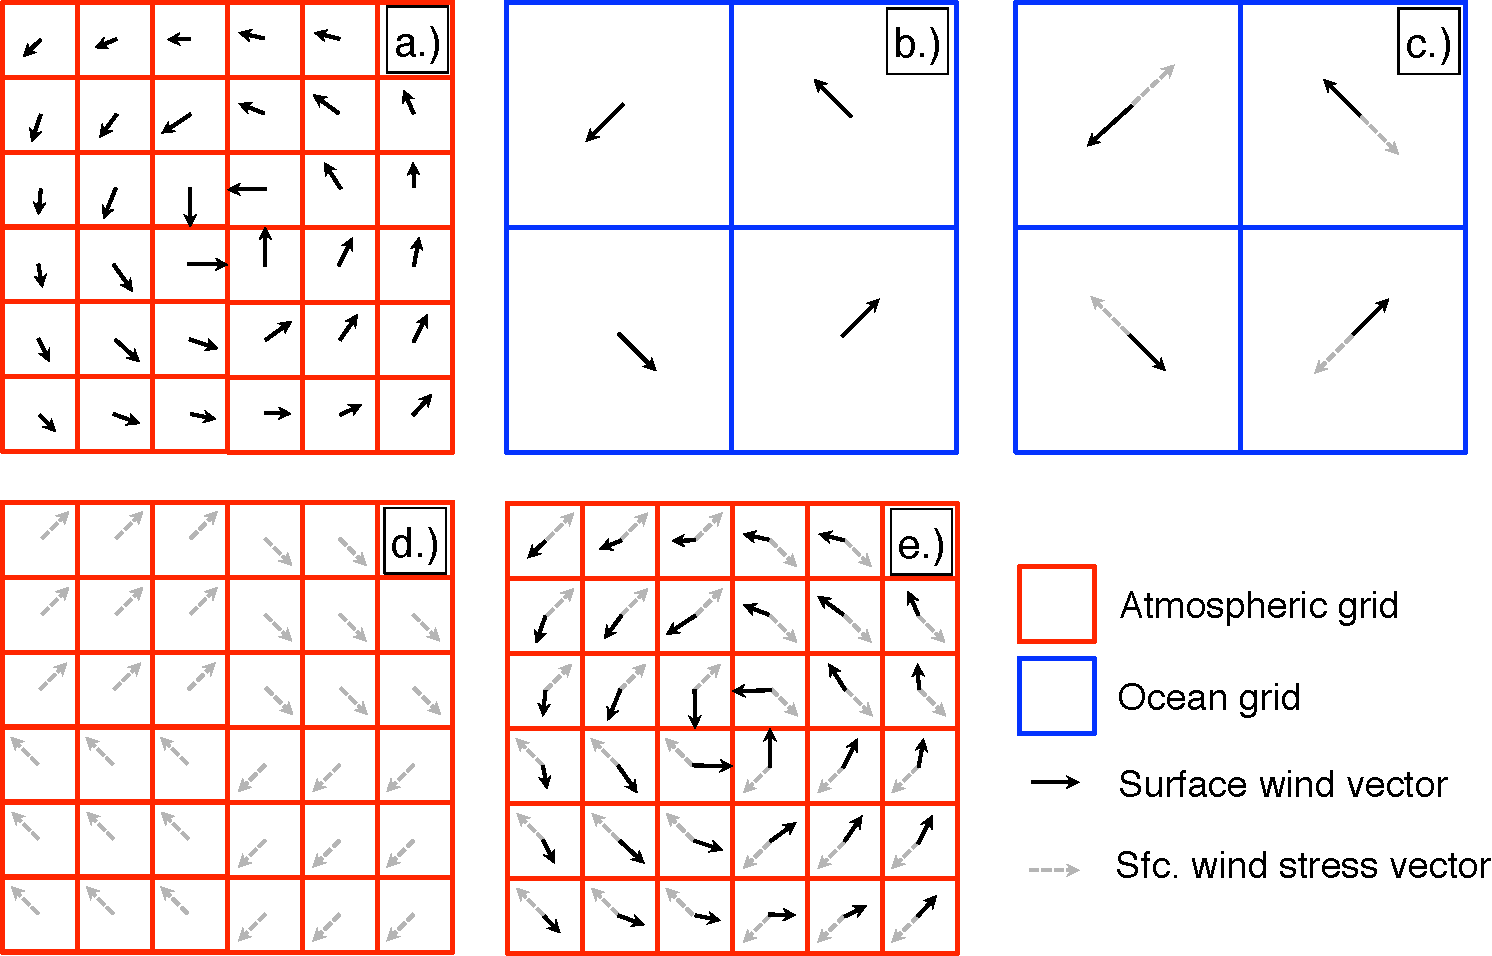
\includegraphics[width=0.8\linewidth]{fig_coupling-schematic.pdf}
\caption{Coupling procedure in CESM. Red (blue) boxes indicate atmospheric (ocean) grid cells. Black (Gray) solid (dashed) vectors show surface wind (wind stress) vectors.}
\label{fig:coupling-schematic}
\end{figure}

\begin{figure}
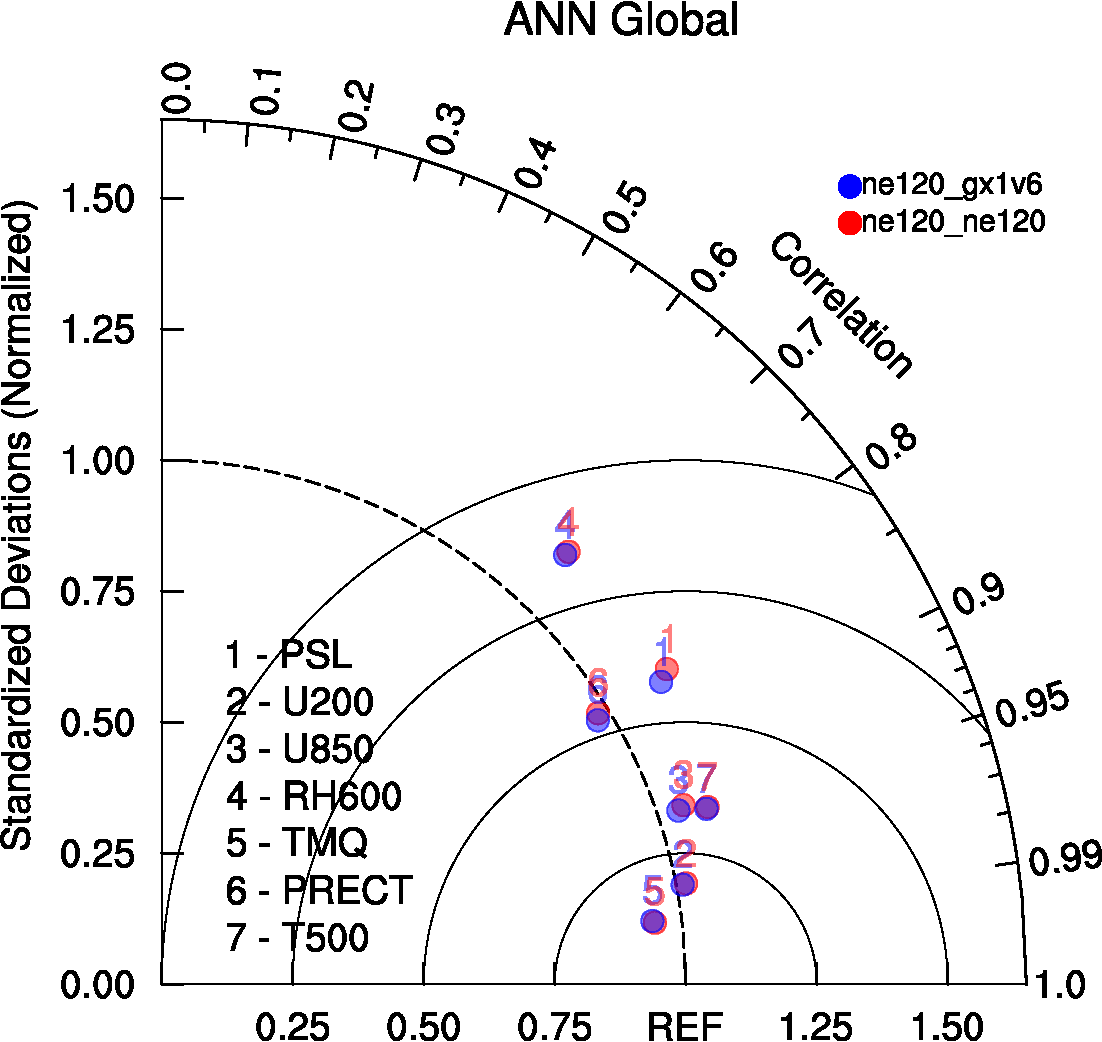
\includegraphics[width=0.7\linewidth]{fig_taylor_globe_ANN.pdf}
\caption{Taylor diagram for globally- and annually-averaged climate statistics. Blue circles represent the results from AMIP simulation coupled to 1\degree{} ocean grid (ne120\_gx1v6) and red circles represent the same for simulation using 0.25\degree{} ocean grid (ne120\_ne120). See text for description of the diagram and explanation of acronyms.}
\label{fig:taylor_global}
\end{figure}

\begin{figure}
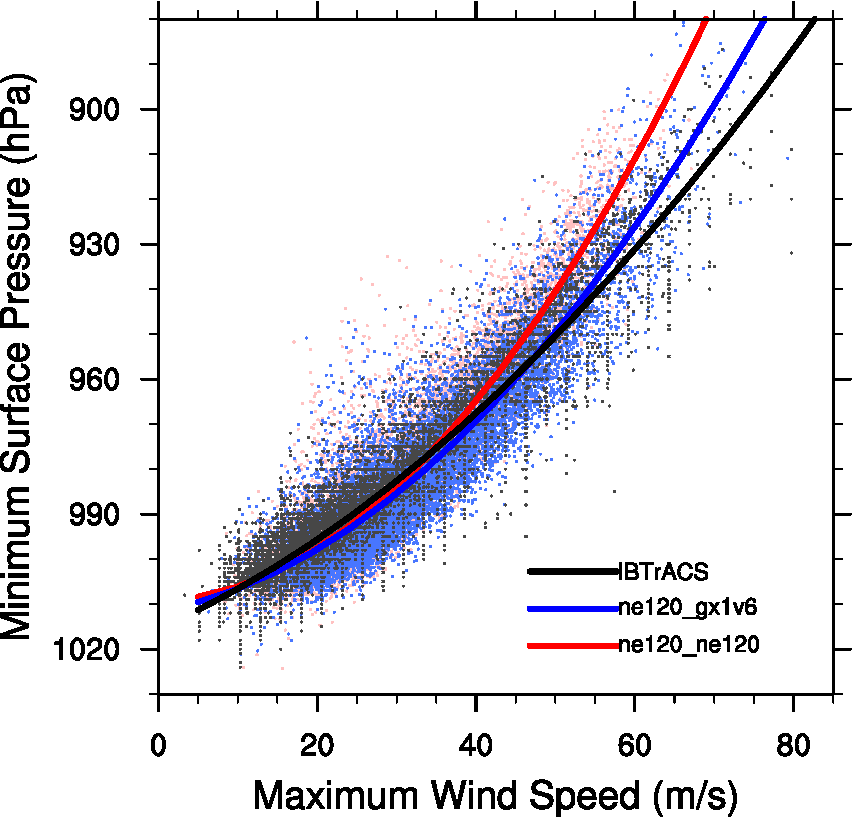
\includegraphics[width=0.8\linewidth]{fig_preswind.pdf}
\caption{Storm minimum surface pressure vs. maximum wind speed relationship with quadratic least squares fit (solid lines) for the CAM5 simulations and IBTrACS observations from 1980 to 2005. Note that 3-hourly output is used for the model simulations, while the IBTrACS data is 6-hourly.}
\label{fig:preswind}
\end{figure}

% Note, for EPS we have to use epstopdf. Update the eps figure but when we submit we'll need to submit pdf. Should update automatically if you put eps in here (might take an extra compile to run through the convertor).
\begin{figure}
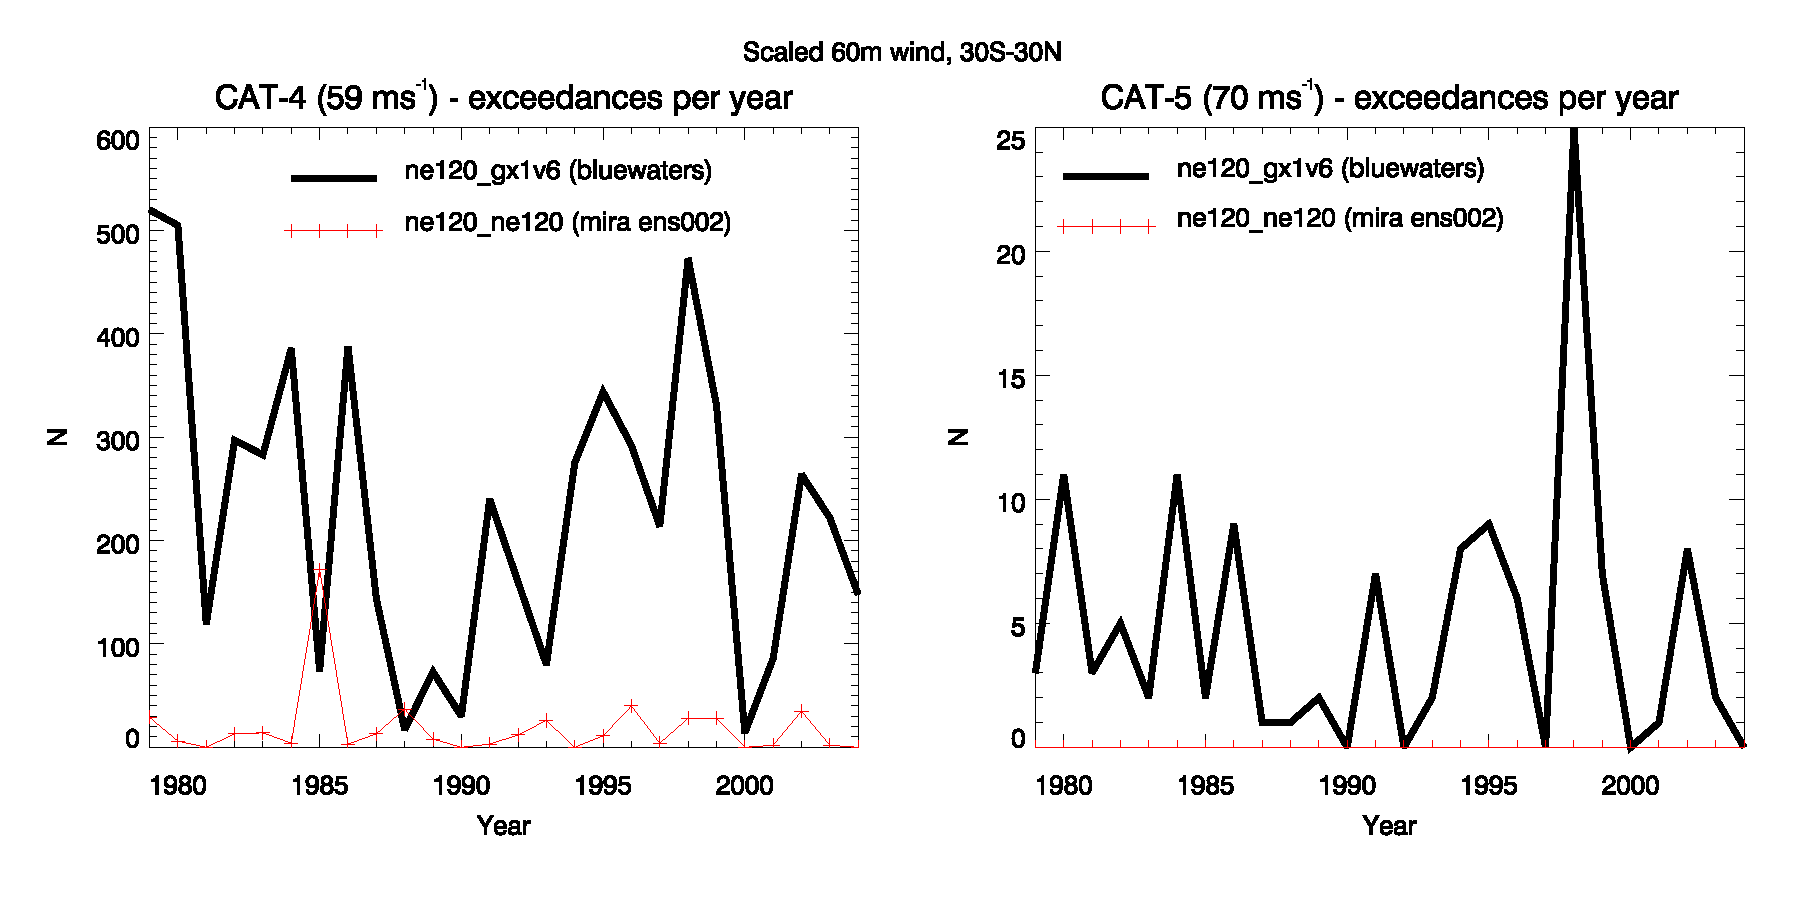
\includegraphics[width=0.8\linewidth]{fig_Maxwind-exceedance.eps}
\caption{Number of TC surface wind instances exceeding category 4 and category 5 wind thresholds for AMIP simulation coupled to 1\degree{} ocean grid (ne120\_gx1v6) and 0.25\degree{} ocean grid (ne120\_ne120). Instances are calculated using 3-hourly data.}
\label{fig:wind-pdfs}
\end{figure}

\begin{figure}
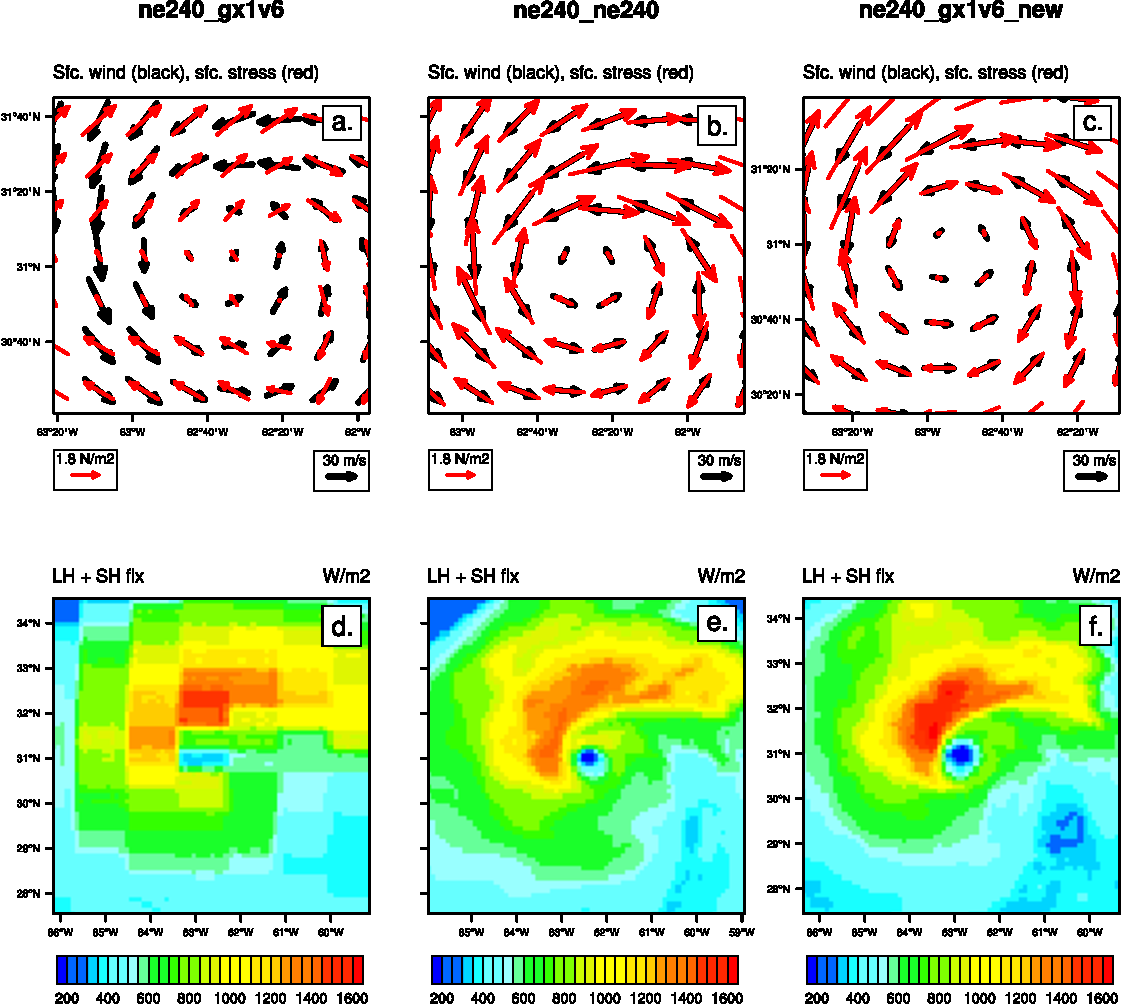
\includegraphics[width=0.7\linewidth]{fig_compareStress.pdf}
\caption{120-hour CAM-SE forecast for Hurricane Leslie, valid at 00Z on September 5th, 2012. Left panels (a,c) are results from forecast using 1\degree{} ocean grid. Right panels (b,d) show results using 0.125\degree{} ocean grid. Top panels (a-b) display instantaneous wind in the lowest model (black vectors) with corresponding lowest model level wind stress (red vectors). Lower panels (c-d) show total surface flux (latent plus sensible heat).}
\label{fig:forecast_panels}
\end{figure}

\begin{table}
\caption{Annual frequency of global tropical cyclones that reach tropical storm (cat. 0-5), hurricane (cat. 1-5) and major hurricane (cat. 4-5) strength the CAM5 simulations and IBTrACS observations for the time period of 1980 to 2005.}\label{tc_counts}
\begin{tabular}{l c c c}
\hline
\textbf{Simulation} & \textbf{Total Storms} & \textbf{Hurricanes} & \textbf{Major Hurricanes}\\
\hline
IBTrACS         & 91.6 $\pm$ 8.5    & 47.1 $\pm$ 5.5 & 10.7 $\pm$ 3.3 \\
ne120$\_$gx1v6 &  70.1 $\pm$ 9.0   & 55.5 $\pm$ 7.7  & 12.5 $\pm$ 3.4\\
ne120$\_$ne120 & 73.2 $\pm$ 10.5  & 50.3 $\pm$ 8.2 & 4.2   $\pm$ 1.9 \\
\hline
\end{tabular}
\end{table}

\end{document}

%%%%%%%%%%%%%%%%%%%%%%%%%%%%%%%%%%%%%%%%%%%%%%%%%%%%%%%%%%%%%%%

More Information and Advice:

%% ------------------------------------------------------------------------ %%
%
%  SECTION HEADS
%
%% ------------------------------------------------------------------------ %%

% Capitalize the first letter of each word (except for
% prepositions, conjunctions, and articles that are
% three or fewer letters).

% AGU follows standard outline style; therefore, there cannot be a section 1 without
% a section 2, or a section 2.3.1 without a section 2.3.2.
% Please make sure your section numbers are balanced.
% ---------------
% Level 1 head
%
% Use the \section{} command to identify level 1 heads;
% type the appropriate head wording between the curly
% brackets, as shown below.
%
%An example:
%\section{Level 1 Head: Introduction}
%
% ---------------
% Level 2 head
%
% Use the \subsection{} command to identify level 2 heads.
%An example:
%\subsection{Level 2 Head}
%
% ---------------
% Level 3 head
%
% Use the \subsubsection{} command to identify level 3 heads
%An example:
%\subsubsection{Level 3 Head}
%
%---------------
% Level 4 head
%
% Use the \subsubsubsection{} command to identify level 3 heads
% An example:
%\subsubsubsection{Level 4 Head} An example.
%
%% ------------------------------------------------------------------------ %%
%
%  IN-TEXT LISTS
%
%% ------------------------------------------------------------------------ %%
%
% Do not use bulleted lists; enumerated lists are okay.
% \begin{enumerate}
% \item
% \item
% \item
% \end{enumerate}
%
%% ------------------------------------------------------------------------ %%
%
%  EQUATIONS
%
%% ------------------------------------------------------------------------ %%

% Single-line equations are centered.
% Equation arrays will appear left-aligned.

Math coded inside display math mode \[ ...\]
 will not be numbered, e.g.,:
 \[ x^2=y^2 + z^2\]

 Math coded inside \begin{equation} and \end{equation} will
 be automatically numbered, e.g.,:
 \begin{equation}
 x^2=y^2 + z^2
 \end{equation}

% IF YOU HAVE MULTI-LINE EQUATIONS, PLEASE
% BREAK THE EQUATIONS INTO TWO OR MORE LINES
% OF SINGLE COLUMN WIDTH (20 pc, 8.3 cm)
% using double backslashes (\\).

% To create multiline equations, use the
% \begin{eqnarray} and \end{eqnarray} environment
% as demonstrated below.
\begin{eqnarray}
  x_{1} & = & (x - x_{0}) \cos \Theta \nonumber \\
        && + (y - y_{0}) \sin \Theta  \nonumber \\
  y_{1} & = & -(x - x_{0}) \sin \Theta \nonumber \\
        && + (y - y_{0}) \cos \Theta.
\end{eqnarray}

%If you don't want an equation number, use the star form:
%\begin{eqnarray*}...\end{eqnarray*}

% Break each line at a sign of operation
% (+, -, etc.) if possible, with the sign of operation
% on the new line.

% Indent second and subsequent lines to align with the first character following the equal sign on the first line.

% Use an \hspace{} command to insert horizontal space into your equation if necessary. Place an appropriate unit of measure between the curly braces, e.g. \hspace{1in}; you may have to experiment to achieve the correct amount of space.


%% ------------------------------------------------------------------------ %%
%
%  EQUATION NUMBERING: COUNTER
%
%% ------------------------------------------------------------------------ %%

% You may change equation numbering by resetting
% the equation counter or by explicitly numbering
% an equation.

% To explicitly number an equation, type \eqnum{}
% (with the desired number between the brackets)
% after the \begin{equation} or \begin{eqnarray}
% command.  The \eqnum{} command will affect only
% the equation it appears with; LaTeX will number
% any equations appearing later in the manuscript
% according to the equation counter.
%

% If you have a multiline equation that needs only
% one equation number, use a \nonumber command in
% front of the double backslashes (\\) as shown in
% the multiline equation above.

%% ------------------------------------------------------------------------ %%
%
%  SIDEWAYS FIGURE AND TABLE EXAMPLES
%
%% ------------------------------------------------------------------------ %%
%
% For tables and figures, add \usepackage{rotating} to the paper and add the rotating.sty file to the folder.
% AGU prefers the use of {sidewaystable} over {landscapetable} as it causes fewer problems.
%
% \begin{sidewaysfigure}
% \includegraphics[width=20pc]{samplefigure.eps}
% \caption{caption here}
% \label{label_here}
% \end{sidewaysfigure}
%
% \begin{sidewaystable}
% \caption{}
% \begin{tabular}
% Table layout here.
% \end{tabular}
% \end{sidewaystable}